% Etapes de conception, insister sur :
% architecture, choix, caractéristiques finales du système implanté

Nous allons présenter dans cette partie les principales étapes de conception
de notre réseau de neurones en détaillant tous les blocs réalisés et les choix
faits à propos de leur architecture.

\subsection{Programme de référence}
% Description du programme de référence en C, de l'utilisation de la base
% de données MNIST, du script en Python, des tableaux contenant les données,
% du taux d'erreur.
Le programme de référence implémente le même réseau de neurones que notre IP
mais directement en C. On peut ainsi l'executer sur un PC ou un micro-processeur 
et comparer les résultats avec l'implémentation réelle sur FPGA. On comparera
la valeur des résultats de sortie et le temps d'exécution entre software et
hardware.

\subsubsection{L'algorithme}

\begin{algorithm}
	\SetAlgoLined
	\For {$f \leftarrow 0$ \KwTo $frames$} {
		$out1[neurons] \leftarrow 0$\;
		$out2[10] \leftarrow 0$\;
		\For {$r \leftarrow 0$ \KwTo $rows$} {
			\For {$c \leftarrow 0$ \KwTo $columns$} {
				\For {$n \leftarrow 0$ \KwTo $neurons$} {
					$out1[n] \leftarrow out1[n] + \texttt{get\_pixel(}f, r, j\texttt{)} \times w1[n][r][c]$\;
				}
			}
		}
		\For {$n \leftarrow 0$ \KwTo $neurons$} {
			$out1[n] \leftarrow \texttt{cut(}out1[n]\texttt{)}$\;
			$out1[n] \leftarrow out1[n] + b1[n]$\;
			\If {$out1[n] < 0$} {
				$out1[n] \leftarrow 0$\;
			}
			$out1[n] \leftarrow \texttt{cut(}out1[n]\texttt{)}$\;
		}
		\For {$n \leftarrow 0$ \KwTo $neurons$} {
			\For {$i \leftarrow 0$ \KwTo $9$} {
				$out2[i] \leftarrow out2[i] + out1[n] \times w2[i][n]$\;
			}
		}
		\For {$i \leftarrow 0$ \KwTo $9$} {
			$out2[n] \leftarrow \texttt{cut(}out2[n]\texttt{)}$\;
			$out2[n] \leftarrow out2[n] + b2[n]$\;
			$out2[n] \leftarrow \texttt{cut(}out2[n]\texttt{)}$\;
		}
		$\texttt{assert(max(}out2\texttt{)} == \texttt{get\_label(}f\texttt{))}$\;
	}
	\caption{Boucle de calcul principal du réseau de neurone logiciel}
	\label{fig:soft_nn}
\end{algorithm}

L'algorithme~\ref{fig:soft_nn} page~\pageref{fig:soft_nn} implémente un réseau de neurones à deux étages.
Chaque étage réalise des multiplications et accumulations pour chaque pixel de
chaque image avec des poids, spécifiques à chaque neurone. Après chaque étage,
le résultat de chaque neurone est additionné avec une constante.

\subsubsection{Les données à traiter dans le réseau}

La configuration actuelle de ce réseau de neurone est adaptée pour la
reconnaissance de chiffres manuscrits de la base de données MNIST\cite{lecun2010mnist}. Une image
en entrée ($28 \times 28$ pixels) correspond à un chiffre manuscrit de 0 à 9.
Le but de ce réseau de neurone est de reconnaître et d'identifier le chiffre
d'une image. Pour une image donnée, le chiffre identifié par le réseau correspond
au numéro du neurone de sortie qui a la plus grande valeur. \\
Dans ce modèle logiciel, les pixels sont encodés sur un octet, les poids et les
constantes sont sur 2 octets. Afin que dans le pire cas, aucune information ne
soit perdue lors de l'accumulation aux différents étages, on réalise cette opération sur
8 octets. Cependant, afin que le logiciel de référence reproduise le même
comportement que notre IP, on ne peut faire transiter entre deux étages uniquement
des données sur 4 octets. C'est
le rôle de la fonction \texttt{cut} qui permet de passer de 64 à 32 bits tout
en conservant le signe.
Notre IP garde uniquement les 32 bits de poids faible de ce mot de 64 bits,
cependant des essais en software pour 100 et 200 neurones ont permis de découvrir
des meilleurs masques qui augmentaient le taux de succès jusqu'à $0.5\%$
(table
\ref{fig:masques} page~\pageref{fig:masques}).

\begin{table}[h!]
\centering
	\begin{tabular}{| l | l | l |}
	\hline
	Masque & Taux de succès (100 neurones) & Taux de succès (200 neurones)\\ \hline
	\texttt{0x00000000FFFFFFFF} & 93.8 & 94.4 \\ \hline
	\texttt{0x00000007FFFFFFF8} & 93.9 & 94.5 \\ \hline
	\texttt{0x0000000FFFFFFFF0} & 93.9 & 94.7 \\ \hline
	\texttt{0x0000001FFFFFFFE0} & 94.3 & 94.8 \\ \hline
	\texttt{0x0000003FFFFFFFC0} & 79.4 & 89.4 \\ \hline
	\texttt{0x000000FFFFFFFF00} & 8.5  & 8.5  \\ \hline
	\end{tabular}
	\caption{Essais de différents masques et leur taux d'erreur}
	\label{fig:masques}
\end{table}

En choisissant un autre masque que
\texttt{0x00000000FFFFFFFF}
il est nécessaire d'effectuer un décalage à droite ensuite.

\subsubsection{Mise en forme des données MNIST}

Les poids des neurones et les constantes des étages de recodage
pour l'application MNIST\cite{lecun2010mnist}, que nous utilisons dans
le logiciel de référence et dans notre IP nous ont été fournis au début du projet
sous forme de fichier texte où sont présentes toutes les données, séparées par
des virgules, et où chaque ligne correspond à un neurone. Un script Python nous
a permis d'analyser ces fichiers pour récupérer les données utiles et de les
replacer dans un unique fichier créé \texttt{net.c} avec les définitions de
4 tableaux d'entiers. Ce fichier est inclus et compilé dans le logiciel de référence et
pour le logiciel embarqué; ainsi les poids et les constantes sont
facilement accessibles depuis le logiciel. \\
Concernant les images, nous les avons récupérées à partir du site
officiel MNIST \linebreak (\texttt{yann.lecun.com/exdb/mnist/}) sous forme de fichiers
binaires où 1000 images de taille $28 \times 28$ pixels sont représentées comme
des tableaux d'octets en C. Un autre fichier binaire nous permet de connaître
le résultat, c'est-à-dire le digit, de chacune de ces images afin de comparer le
résultat de notre réseau de neurones avec le résultat attendu.
Les fonctions \texttt{get\_pixel} et \texttt{get\_label} permettent d'obtenir
facilement ces informations depuis le logiciel.

\subsubsection{Les résultats}

Les résultats du logiciel de référence en sortie de chacun des niveaux nous
sont utiles pour les comparer avec ceux de notre IP et s'assurer que les calculs
sont justes pour la classification des images MNIST\cite{lecun2010mnist}. On s'attend à trouver
un même taux d'erreur ($93.80\%$) car les configurations sont identiques
mais un calcul beaucoup plus rapide de toutes les images.



\subsection{IP du réseau de neurones}

\begin{figure}[h!]
	\begin{center}
		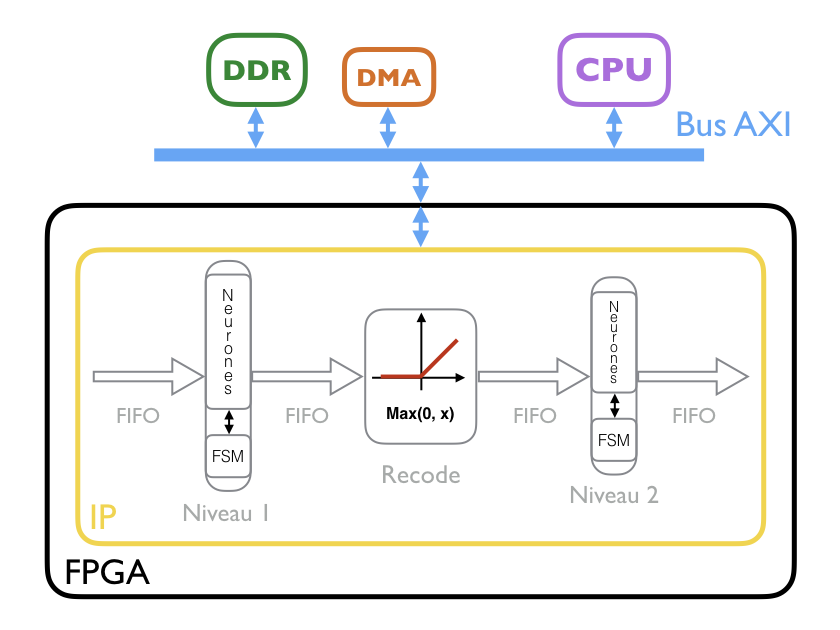
\includegraphics[scale=0.4]{NNSchema}
		\label{fig:NNSchema}
		\caption{Schéma de l'IP réseau de neurones dans son environnement }
	\end{center}
\end{figure}

\subsubsection{Le neurone}
	Le neurones est l'élément de base de notre réseau.
	C'est donc la première chose que nous avons implémenté.
	Pour faire cela, nous avons pensé le neurone en terme de
	fonctionnalités uniquement.
	Nous allons donc décrire ici la façon dont nous avons conçu un neurone.
	Un neurone a deux modes de fonctionnement.
	Le premier est le mode de chargement des poids en mémoire, le second
	est le mode de calcul.

	\paragraph{Le mode de chargement des poids\\}

	Pour permettre aux neurones d'accomplir leur rôle principale, il faut que chaque neurone ait
	accès à ses poids. Etant donné que chaque neurone doit disposer de ses propres poids
	(identiques pour une application donnée et donc pour une grandes quantité d'images)
	il est donc préférable que chaque neurone les mémorise. Afin d'accomplir cela,
	les neurones reçoivent une adresse (numero du poids à mémoriser) ainsi qu'un poids.
	Alors le neurone peut mémoriser le poids présent sur son entrée dans
	sa BRAM à l'adresse reçue à condition que ce neurone possède le {\em token} de
	configuration et qu'il reçoive le signal lui indiquant qu'un poids est présent sur son entrée.\\
	Le token de configuration est passé de neurone en neurone
	sur ordre du signal de contrôle pour qu'ils se configurent l'un après l'autre.
	Vous trouverez une illustration de ce fonctionnement en
	figure~\ref{fig:N_poids} page~\pageref{fig:N_poids}.
	\begin{figure}[h!]
		\begin{center}
			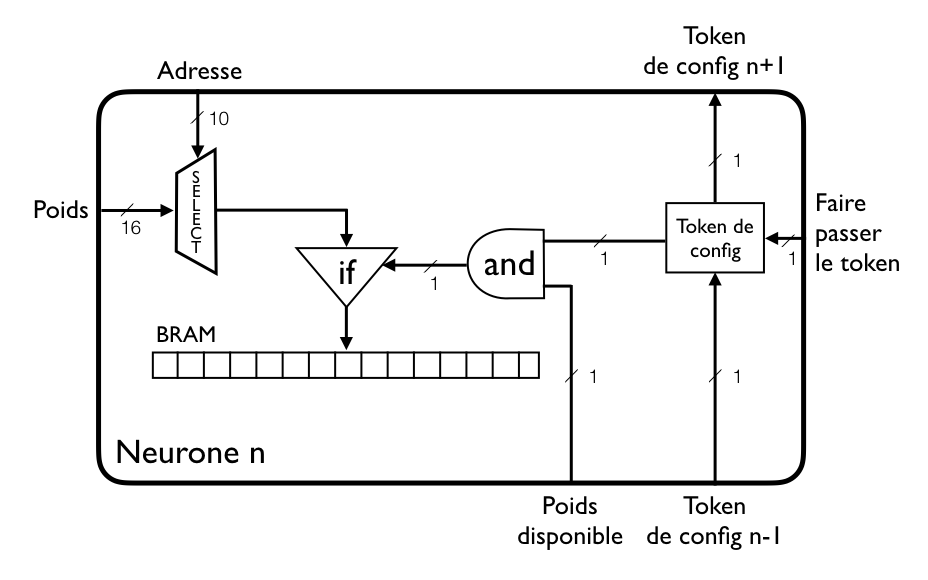
\includegraphics[scale=0.4]{N_poids}
			\caption{Schéma fonctionnel de l'implémentation du neurone en mode de configuration}
			\label{fig:N_poids}
		\end{center}
	\end{figure}

	\paragraph{Le mode de calcul\\}
	\begin{figure}[h!]
		\begin{center}
			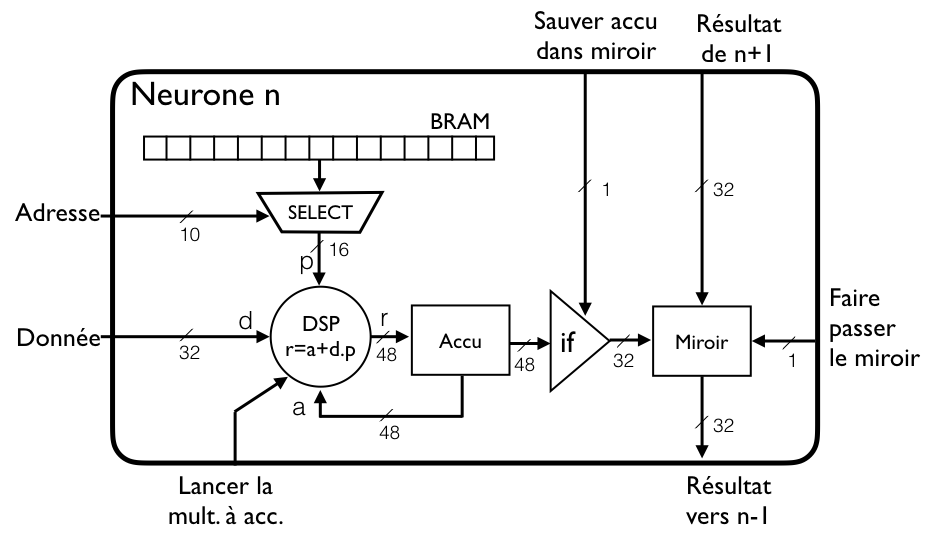
\includegraphics[scale=0.4]{N_calcul}
			\caption{Schéma fonctionnel de l'implémentation du neurone en mode de calcul}
			\label{fig:N_calcul}
		\end{center}
	\end{figure}

	Le mode de calcul est le mode principal d'un neurone. C'est dans ce mode que le neurone
	reçoit des données et qu'il effectue une succession de multiplications à accumulations entre
	la valeur du pixel reçu et le poids correspondant à l'adresse qui lui est donné. L'opération clé
	d'un neurone peut être écrite comme :
	$$\sum_{adr=0}^n p_{adr}*d$$
	avec $n$ données entrantes dans le réseau, $p_{adr}$ le poids à l'adresse $adr$
	et $d$ la donnée entrante.

	En effectuant cette opération sur chaque pixel d'une image, un neurone du premier niveau du réseau
	est capable de produire un résultat par image. Les neurones des niveaux suivant ne reçoivent
	pas des pixels mais les résultats du niveaux précédent et opère de la même façon pour enfin
	produire chacun un résultat (voir figure~\ref{fig:N_calcul} page~\pageref{fig:N_calcul}).
	\\{\em Notez qu'entre deux niveaux les résultats passent par l'étage de recode
	(cf. Partie~\ref{plan:recode} "L'étage de recodage")}.

	Une fois que chaque neurone a produit son résultat, ils vont en faire une copie dans
	un registre appelé {\em miroir} et remettre le registre d'accumulation à 0. Ainsi,
	le calcul de l'image suivante pourra être commencé alors que résultat de l'image précédente
	sera évacué vers la FIFO de sortie suivante. Pour ce faire, à la réception du signal
	{\em sauver accu dans miroir}, chaque neurone va faire passer la valeur de son
	registre miroir au neurone suivant et récupérer la valeur du neurone précédent.
	Cela permet de ne connecter qu'un neurone à la FIFO
	et de faire évacuer les données les unes après les autres dans la FIFO
	(voir figure~\ref{fig:N_calcul} page~\pageref{fig:N_calcul}).

\subsubsection{La machine à états (FSM) du niveau de neurones}

La machine à états ou FSM (Finite State Machine) contrôle l'ensemble des neurones
d'un niveau de neurones.
Elle a été conçue de façon à contrôler un nombre de neurones indéfini : qu'il y
ait 1 ou 100000 de neurones, la machine à états reste la même.

Les signaux de contrôle de la FSM sont reliés à tous les neurones.

Pour des raisons de simplicité le contrôle des neurones est séparé en deux
machines à états qui communiquent entre elles par le biais d'un drapeau.

\paragraph{La machine à états de contrôle des neurones\\}

L'ensemble de cette machine à états est visible dans la
figure~\ref{fig:fsm}~page~\pageref{fig:fsm}.

Dans le mode accumulation,
il n'y a pas besoin de distinguer chaque neurone, on se contente donc d'envoyer
les signaux de contrôle à tous les neurones.
Dans le mode chargement des poids de neurones, il faut être capable de commander
un neurone à la fois. Pour cela, la FSM génère un token de configuration au début
de la phase de chargement des poids et le donne au premier neurone. Sans ce token,
le neurone est inactif dans cette phase. Une fois que la machine à états a fini de
charger les poids d'un neurone, elle déclenche un décalage du token de configuration
entre les neurones. Une fois le dernier neurone atteint, le décalage du token
le renvoie sur la FSM qui sait donc qu'elle a fini de configurer l'ensemble des
neurones.

\begin{sidewaysfigure}
	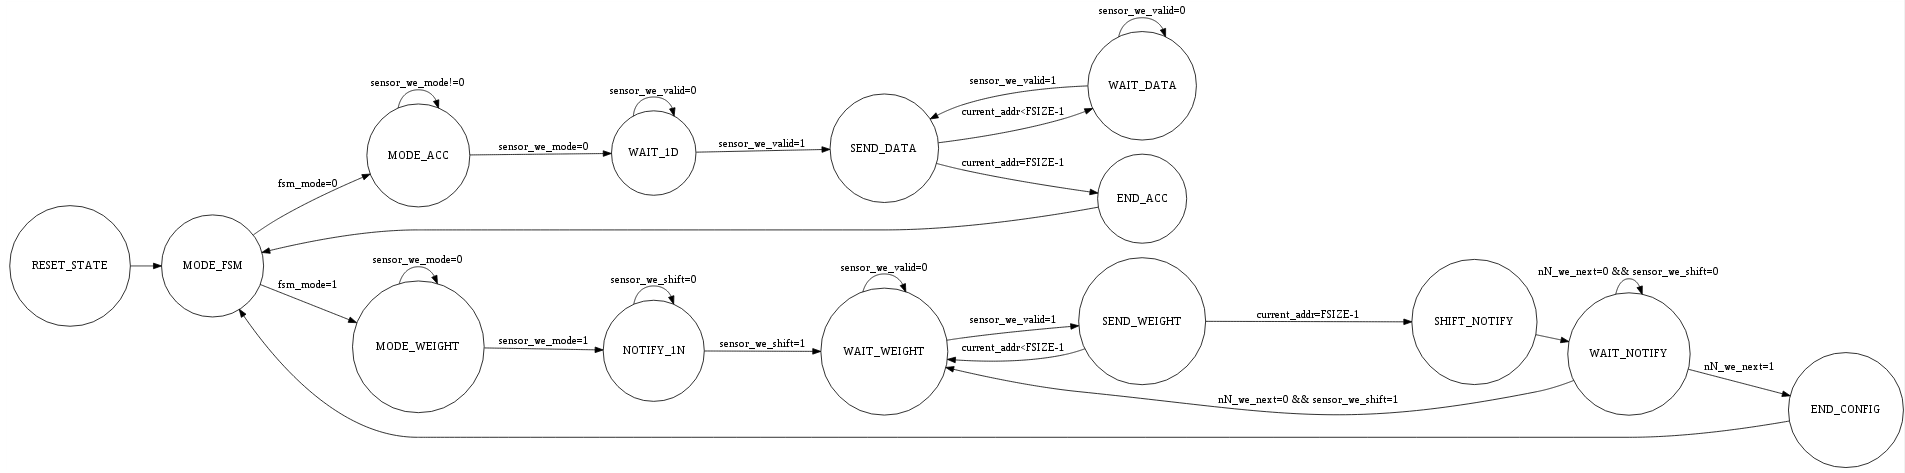
\includegraphics[width=\textwidth]{fsm}
	\caption{Machine à états de contrôle des neurones}
	\label{fig:fsm}
\end{sidewaysfigure}

Voici de courtes explications pour les différents états:
\begin{itemize}
	\item \verb+RESET_STATE+: état de reset
	\item \verb+FSM_MODE+: choix du mode de fonctionnement du niveau de
		neurones, soit chargement des poids, soit accumulation.
	\item \verb+MODE_ACC+: on est en mode accumulation, on le signale aux
		neurones, et on attend qu'ils aient pris en compte le changement.
	\item \verb+WAIT_1D+: on attend que la première donnée soit présente
		dans la FIFO d'entrée pour commencer l'accumulation.
	\item \verb+SEND_DATA+: accumulation des neurones. Si jamais on a atteint
		la fin d'une image on le notifie à la machine à états de la
		chaîne de miroir, sinon on attend une nouvelle donnée.
	\item \verb+WAIT_DATA+: on attend une nouvelle donnée
	\item \verb+END_ACC+: on a fini l'accumulation sur une image, on retourne
		dans l'état de choix de mode de la FSM.
	\item \verb+MODE_WEIGHT+: on est en mode chargement des poids, on le signale aux
		neurones, et on attend qu'ils aient pris en compte le changement.
	\item \verb+NOTIFY_1N+: on passe le token de configuration au premier neurone
		et on attend qu'il nous confirme sa réception.
	\item \verb+SEND_WEIGHT+: chargement du poids dans la mémoire du neurone.
		Si jamais on a atteint la fin d'un neurone, on décale le token
		de configuration, sinon on attend un nouveau poids.
	\item \verb+WAIT_WEIGHT+: on attend un nouveau poids.
	\item \verb+SHIFT_NOTIFY+: on décale le token de configuration.
	\item \verb+WAIT_NOTIFY+: on attend que les neurones aient bien décalé
		le token de configuration, si jamais la FSM le reçoit cela signifie
		que l'on a configuré tous les neurones, dans ce cas on passe en
		fin de configuration, sinon on continue de configurer les neurones suivants.
	\item \verb+END_CONFIG+: on a fini le chargement des poids, on retourne
		dans l'état de choix de mode de la FSM.
\end{itemize}


\paragraph{La machine à états de la chaîne de miroirs\\}

L'ensemble de cette machine à états est visible dans la
figure~\ref{fig:fsm_miroir}~page~\pageref{fig:fsm_miroir}.
Elle est chargée de décaler les miroirs de la chaîne de miroirs des neurones
pour les transmettre à la FIFO de sortie.

\begin{figure}[h!]
	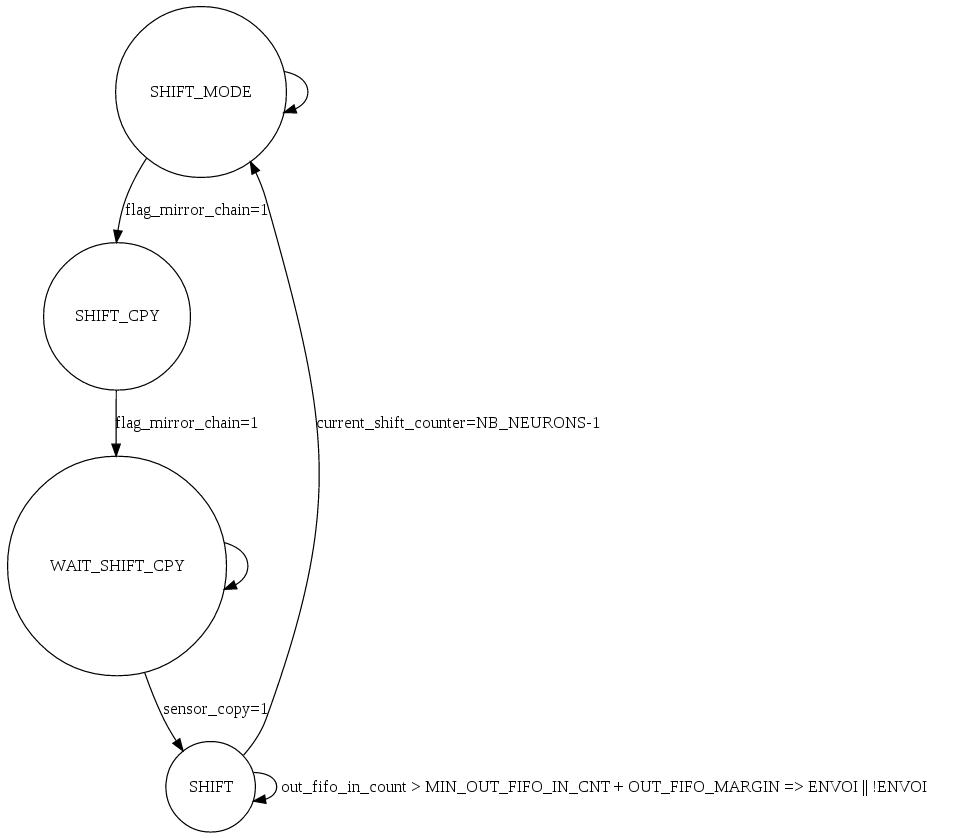
\includegraphics[width=\textwidth]{fsm_miroir}
	\caption{Machine à états de la chaîne de miroir}
	\label{fig:fsm_miroir}
\end{figure}

Voici de courtes explications pour les différents états:
\begin{itemize}
	\item \verb+SHIFT_MODE+: état d'attente, si la FSM de contrôle des neurones
		passe le drapeau de communication à 1, il faut commencer à décaler
		la chaîne de miroir.
	\item \verb+SHIFT_CPY+: copie de la valeur des registres d'accumulation
		de chaque neurone dans leur miroir respectif.
	\item \verb+WAIT_SHIFT_CPY+: on attend que les neurones aient copiés leur
		registre dans le miroir.
	\item \verb+SHIFT+: on décale les miroirs de chaque neurone dans le neurone suivant
		uniquement s'il y a suffisamment de place dans la FIFO de sortie. On prend en compte
		le temps de propagation des signaux de contrôle pour qu'il n'y ait pas de donnée perdues
		à cause d'un manque de place dans la FIFO de sortie.
\end{itemize}


\subsubsection{Le niveau de neurones}
% TODO: inclure la figure en question
Le niveau de neurones est l'entité de notre IP qui regroupe un certain nombre
de neurones (100 ou 200 pour le premier niveau, 10 pour le deuxième) et une
machine à états afin de les contrôler. \\
Afin de pouvoir relier les signaux de contrôle de la machine à états à plus de
100 ou 200 neurones, de simples fils auraient posés
problème. En effet, pour deux neurones très éloignés dans le FPGA, les temps
de propagation des données envoyées en même temps de la FSM n'auraient pas été
identiques et cela aurait créé des problèmes de synchronisation. Pour cela, nous
avons utilisé des buffers de distribution, déjà disponible, pour distribuer les
signaux de contrôle de la FSM à tous les neurones ou les données d'entrée aux neurones. 
Un buffer de distribution est constitué d'un arbre de fils avec la racine connectée à un port de sortie de la FSM et les feuilles
connectées à tous les neurones. Le nombre de fils fils de chaque noeud est un
paramètre du buffer (2 dans la figure~\ref{fig:nnlayer} page~\pageref{fig:nnlayer}). 
L'avantage d'utiliser un buffer de distribution est qu'il certifie que le passage d'un niveau de l'arbre 
prend un cycle. On est alors assuré que la donnée arrivera en même
temps à tous les neurones. \\
Certains signaux se connectent uniquement au premier ou au dernier des neurones
et d'autres entre deux neurones consécutifs, ces connexions sont alors réalisées avec de simples fils. 
Pour gérer ces connexions on instancie tous les neurones grâce à la boucle VHDL :\\
\texttt{gen\_neu: for i in 0 to NBNEU-1 generate} \\
où chacun des ports des neurones sont reliés à des tableaux de signaux pour
faciliter leur utilisation.

\begin{figure}[h!]
	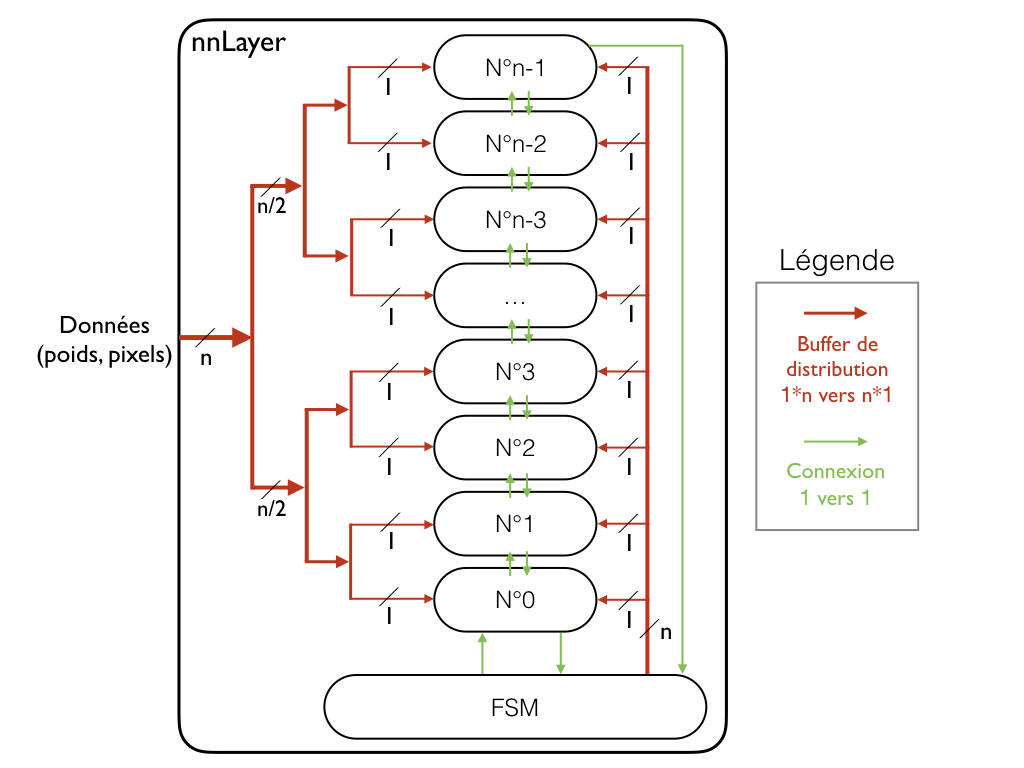
\includegraphics[width=\textwidth]{nnlayer}
	\caption{Schema d'un niveau de recode montrant les différents type 
	d'interconnexion entre les différents éléments le constituant}
	\label{fig:nnlayer}
\end{figure}

\subsubsection{L'étage de recodage}
\label{plan:recode}

Situé après le niveau de neurones, l'étage de recodage possède deux fonctions :
ajouter une constante aux valeurs sortants du niveau de neurones (chaque
constante est propre à un neurone) et
supprimer les valeurs négatives après ajout de constante.

L'étage est contrôlé par une machine à états visible sur la
figure~\ref{fig:recode_fsm}~page~\pageref{fig:recode_fsm}.

\begin{figure}[h!]
	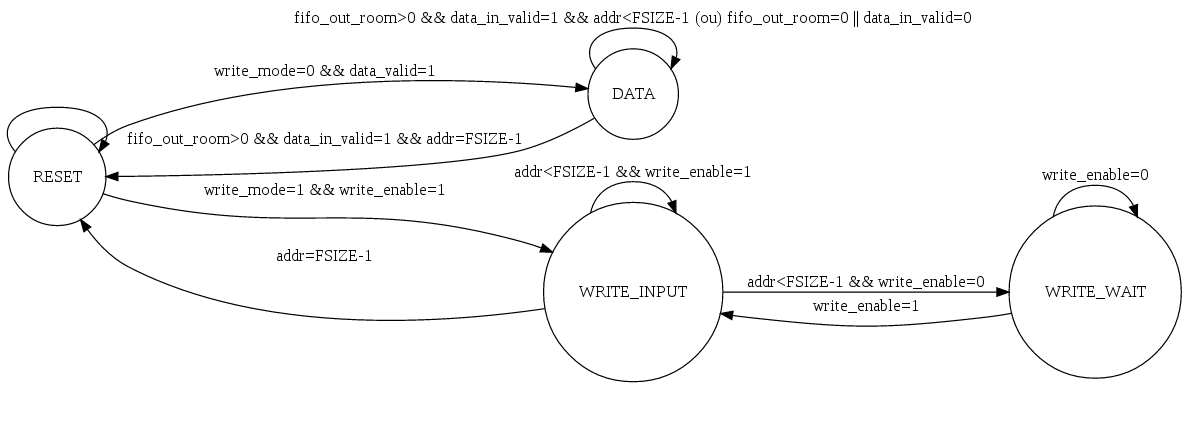
\includegraphics[width=\textwidth]{recode_fsm}
	\caption{Machine à états de l'étage de recodage}
	\label{fig:recode_fsm}
\end{figure}

Voici de courtes explications pour les différents états:
\begin{itemize}
	\item \verb+RESET+: état de choix de mode et d'attente de données présentes.
		Si le mode est le traitement classique et qu'il y a une donnée
		disponible dans la FIFO d'entrée, on passe dans l'état de traitement
		des données. Si il s'agit du mode de chargement des poids
		et qu'il y a un poids disponible dans la FIFO d'entrée, on passe dans l'état
		de chargement des poids.
	\item \verb+WRITE_INPUT+: on écrit le poids dans la mémoire,
		si on a atteint la fin de la mémoire, on repasse dans l'état \verb+RESET+,
		s'il y a une donnée
		disponible ensuite on continue d'écrire les poinds dans la mémoire,
		sinon on attend qu'il y ait un poids disponible.
	\item \verb+WRITE_WAIT+: on attend qu'il y ait un poids disponible.
	\item \verb+DATA+: on effectue le traitement de la donnée en entrée seulement si:
		elle est disponible, il y a de place dans la FIFO de sortie et on n'a pas atteint
		la fin de la totalité des données sortant d'un décalage complet de la chaîne
		de miroirs. Le traitement consiste à ajouter une constante, et supprimer la valeur
		(envoyer 0 en sortie) si la valeur après ajout de constante est négative, sinon on
		envoie la valeur avec l'ajout de constante.
		S'il n'y a pas de place en sortie ou pas de donnée en entrée, on attend que les deux conditions
		soient valides.
		Si on a atteint la fin d'un décalage complet de la chaîne de miroirs, on repasse dans
		l'état de \verb+RESET+.
\end{itemize}

\subsubsection{Le pipeline complet}
Une fois chaque éléments ci-dessus créé, il a fallut les mettre ensemble pour accomplir 
le fonctionnement global du réseau. Il est important de réfléchir à la façon dont ces différents éléments 
échangent leurs données. En effet, les différents organes du réseaux ne doivent pas calculer la même 
quantité de donnée, donc le temps de traitement d'une image n'est pas identique dans tout le réseau. 
C'est pourquoi, entre chaque élément du réseau (entrée, niveau de neurone 1, recodage, niveau 2, sortie) 
nous avons utilisé des FIFOs. Les FIFOs utilisées nous ont été fournies, elles ont une entrée et une sortie sur 32 bits, 
64 cases mémoire de 32 bits, 4 signaux de contrôle et 2 signaux donnant le nombre de places disponibles et occupées. 
Deux des signaux de contrôle permettent à la FIFO d'avertir l'élément suivant qu'une donnée peut être sortie de la FIFO 
et à l'élément précédent  q'une donnée peut être écrite. Les deux autres signaux de contrôle permettent eux aux élément 
d'avertir la FIFO qu'une donnée est lue ou écrite (c'est un signal acquittement). 
L'utilisation des FIFOs du réseau est différente dans les deux modes du réseau.
	\paragraph{Le pipeline en mode chargement des poids}
	Lorsque le réseau de neurones est en mode configuration, chaque élément va récupérer les constantes dans la 
	toute première FIFO. En effet, le DMA va faire un transfert de donnée de la DDR vers la FIFO d'entrée via le bus AXI. 
	En connectant correctement les signaux de contrôle de la première FIFO aux différents éléments du réseau, 
	ils pourront récupérer les données dont ils ont besoin pour le mode de calcul chacun leur tour. 
	(voir. figure~\ref{fig:pipeline_poids} page~\pageref{fig:pipeline_poids})
	
	\begin{figure}[h!]
		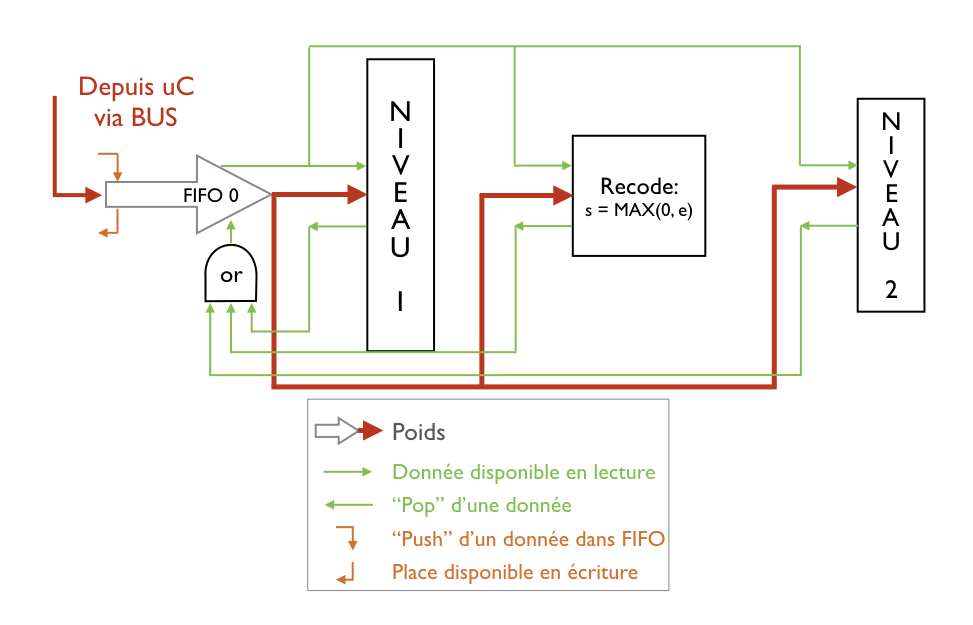
\includegraphics[width=\textwidth]{pipeline_poids}
		\caption{Pipeline du réseau en mode chargement des poids pour illustrer l'utilisation de la FIFO 0}
		\label{fig:pipeline_poids}
	\end{figure}
	
	\paragraph{Le pipeline en mode calcul}
	Lorsque le réseau de neurones est en mode de calcul, les images arrivent pixel par pixel dans la première FIFO. 
	Chaque neurone produit 1 donnée qu'ils envoient une à une dans la FIFO n°2, le recodage traite alors ces 
	données une à une et enfin l'étage 2 reçoit ces résultats en lisant dans la FIFO n°3. La dernière FIFO 
	permet de stocker les données de sortie du réseau afin de les envoyer (par paquets de 16) au micro-processeur. 
	(voir figure~\ref{fig:pipeline_data} page~\pageref{fig:pipeline_data}).
	\begin{figure}[h!]
		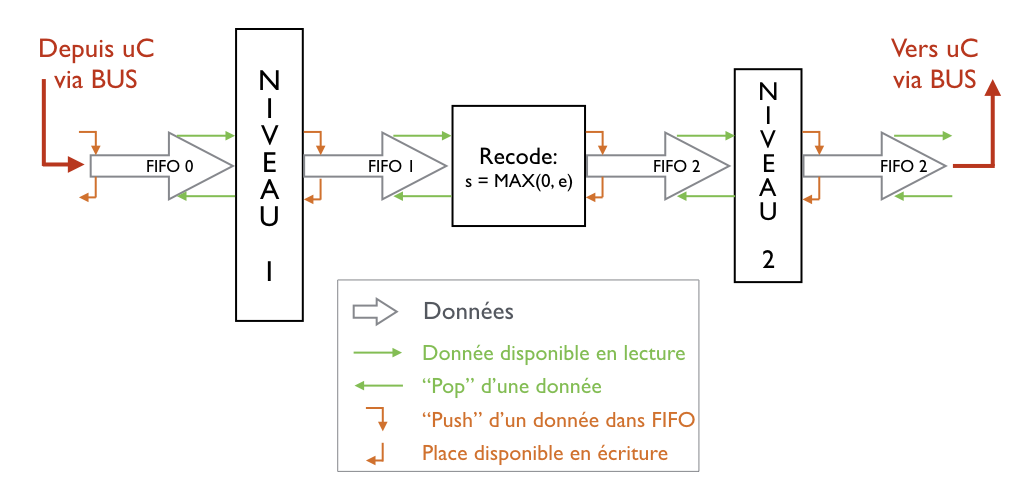
\includegraphics[width=\textwidth]{pipeline_data}
		\caption{Pipeline du réseau en mode de calcul pour illustrer l'utilisation des FIFO dans le réseau}
		\label{fig:pipeline_data}
	\end{figure}

\subsection{Logiciel de commande}
Le logiciel de commande est le logiciel embarqué sur la carte, qui s'execute
sur processeur ARM. Celui ci permet de configurer notre réseau de neurones avec
les poids et les constantes choisies, de lancer les calculs avec les valeurs
voulues et de récupérer les résultats. Il s'écrit en C et s'interface avec
l'utilisateur grâce à la liaison série (composant UART). Le squelette de base
était déjà disponible avec toutes les fonctions nécessaires, le code était
écrit pour la configuration d'un niveau de neurone, l'envoi d'images simples et
la récupération des résultats. Les données
concernant les poids, les constantes, les images et les paramètres (taille d'une
image, nombre de neurones à chaque niveau, nombre d'images) étaient toutes notées
dans un fichier (\texttt{dataset.h}). Nous avons gardé ce fonctionnement pour la
majeure partie de notre projet car il nous a permis de tester facilement notre
IP pour des images de petites tailles, des niveaux de neurones avec très peu
de neurones (3) et de configurer facilement les pixels des images et les poids
choisis pour connaître les résultats attendus et comparer avec ceux de notre IP.
Nous avons cependant complété ce code afin qu'il puisse gérer notre IP complète
avec deux niveaux de neurones et un étage de recodage.
Par la suite, nous avons repris les mêmes données MNIST\cite{lecun2010mnist} que pour le logiciel de
référence afin de tester l'application réelle. \\

\subsubsection{Moyens de communication avec l'IP}
Pour pouvoir échanger des données entre le logiciel embarqué et notre IP, 16
registres de 32 bits peuvent être lus et écrits des deux côtés de notre
système. Par exemple
les 4 premiers bits du registre 3 contiennent la configuration actuelle de notre
IP : mode envoi des images, mode configuration (cad chargement des poids) du
niveau 1, 2 ou de l'étage de recodage. Cette configuration est transmise
aux blocs concernés afin qu'ils changent leur comportement et attendent les
données utiles en entrée. Un autre bit de ce registre permet d'envoyer le
signal \texttt{RESET} à toute notre IP.
Les registres sont accédés avec un offset à partir d'une adresse de base
sur le bus AXI. Des fonctions utilitaires déjà présentes
permettent de faciliter les accès grâce à des masques et des opérations
binaires avec les bons registres. \\
Pour envoyer ou recevoir de plus grosses quantités de données comme l'envoi
des poids ou des frames, ou récolter les résultats de notre réseau de neurones,
on utilise la fonction burst de notre bus AXI. On peut alors transférer des
données de façon rapide entre la DDR où le logiciel alloue de l'espace
pour stocker poids, frames et résultats et les FIFOs d'entrée et de sortie pour
communiquer avec notre réseau de neurones. \\
A chaque fois que l'on souhaite faire un transfert, les mêmes opérations sont
faites :
\begin{itemize}
	\item si c'est une écriture, les données à écrire sont présentes, comme
		variables globales, dans des tableaux multi-dimensions dans un
		fichier C
	\item on alloue un tableau d'entiers (signé pour les poids, non signé
		pour les frames) de 32 bits de manière dynamique. La taille
		du tableau alloué dépend des données considérées mais on alloue
		32 bits (1 case du tableau) par donnée (1 poids, 1 constante ou
		1 pixel d'une frame) afin de faciliter leur traitement par l'IP,
		les FIFOs ayant des cases de même taille.
	\item afin de préparer ce tableau aux bursts, qui sont des transferts
		par bloc
		de 16 mots de 32 bits, soit 16 cases du tableau vers une FIFO,
		on doit aligner son adresse sur des frontières de $16 \times
		4$ octets. On ajoute alors $16 \times 4$ comme supplément à la
		taille nécessaire du tableau et on incrémente l'adresse
		renvoyée par \texttt{malloc} jusqu'à trouver une frontière de
		$16 \times 4$ octets, cad une adresse terminant par
		\texttt{0x00}, \texttt{0x40}, \texttt{0x80} ou \texttt{0xC0}.
		Grâce au supplément dans la taille ajouté, on est sûr d'avoir
		suffisament de place pour écrire les données même après avoir
		incrémenté l'adresse pour l'arrondir.
	\item on écrit les données dans le tableau alloué à partir des
		variables globales déjà présentes
	\item on passe l'adresse de ce tableau à l'IP par un registre
	\item on indique dans un autre registre le nombre de bursts nécessaires
		pour transférer tout le tableau vers la FIFO. Si le tableau n'a
		pas un nombre de case qui est multiple de 16, on fait un burst
		supplémentaire pour inclure le reste. Il faudra alors
		envoyer à l'IP un signal \texttt{RESET} entre deux écritures
		afin de vider les FIFOs de leurs données résiduelles invalides.
\end{itemize}
\subsubsection{Débogage}
% problèmes uniquement liés au soft : printf et GDB
% (allocation et remplissage des tableaux)
Pour déboguer le système global, notre IP avec le logiciel embarqué, nous avons
utilisé différentes manières. \\
Pour des problèmes uniquement liés au logiciel (mauvaise taille, mauvais indices
des tableaux, ...),
nous avons utilisé le composant
UART avec la fonction Xilinx \texttt{printf} pour envoyer par le lien série des
informations sur un terminal distant. En passant par la suite à la carte ZedBoard,
nous avons pu faire fonctionner la fonction Debug sur SDK Xilinx pour pouvoir
avancer pas à pas dans le code et inspecter l'état des variables. \\
% problèmes de l'IP :
% informations contenues dans certains registres
Les problèmes liés à notre IP sont plus difficiles à déboguer car nous ne pouvons
pas simuler le système complet à cause de licences manquantes. Pour repérer
certains problèmes comme des boucles d'attente infinies, des données de
notre IP sont écrites dans des registres comme les signaux \texttt{READY} et
\texttt{ACK} de chacunes des FIFOs et les \texttt{COUNT} pour ces FIFOs. Des
fonctions utilitaires permettent de lire facilement ces informations à partir
des registres concernés et de nous renseigner plus précisément sur quel est
l'étage bloquant de notre système. \\
% fonctions pour poper des valeurs en cours de route
Cependant ces méthodes ne peuvent nous renseigner uniquement sur l'étage qui
fait bloquer tout le système et non pas sur la validité des données produites
en sortie de chaque étage. Une fonctionnalité pour sortir des données de chacune
des FIFOs intermédiaires a alors été implémentée du côté hardware, active à la
lecture d'un certain registre, qui n'était jusque là pas utilisé. La gestion
côté software est correctement effectuée pour attendre qu'il y des données dans
les FIFOs avant de les sortir. Ce mécanisme nous a permis d'isoler les différents
bugs de notre IP à un étage et de pouvoir les corriger individuellement.

\subsection{Caractéristiques finales du système implanté}
Pour étudier les caractéristiques finales de notre système, il est important
de définir les caractéristiques théoriques atteignables.

\subsubsection{Caractéristiques théoriques}

On suppose qu'il n'y a pas de blocage de données en sortie de notre
composant et que des données sont toujours disponibles en entrée.

Ainsi, il faut $2\times FSIZE$ cycles (où $FSIZE$ est la taille d'une image)
pour accumuler les données dans le premier
niveau de neurones. Puis pour accumuler dans le deuxième niveau, il faut
$2\times N_1$ cycles (où $N_1$ est le nombre de neurones dans le premier niveau de
neurones).

De plus, pour décaler les données du premier niveau jusqu'au deuxième
niveau, il faut N1 cycles pour décaler les données dans la FIFO, puis trois cycles
pour que la première donnée traverse les FIFOs et l'étage de recodage, les données
qui suivront n'auront pas de latence. Ainsi Entre le premier niveau de neurones
et le deuxième, il y a $N_1 + 3$ cycles.
Mais le deuxième niveau de neurones va être bloquant (car $2\times N_1 > N_1 +3$
pour $N_1 > 2$). Donc pour que les données soient décalées du premier
niveau de neurones et accumulées par le deuxième, il faut $2\times N_1$ cycles.

Après le deuxième niveau de neurones, il faut $N_2$ cycles (où $N_2$
est le nombre de neurones dans le deuxième niveau) pour décaler les données.

Ainsi le nombre de cycles requis pour traiter une image est:
\begin{equation}
	N_{calcul} = N_1 \times 2 + FSIZE \times 2 + N_2
\end{equation}

Donc le temps de calcul d'une image est:
\begin{equation}
	T_{calcul} = N_{calcul}/f_{réseau\_de\_neurones}
\end{equation}

Néanmoins, si nous avions optimisé la machine à états de contrôle des neurones pour
qu'elle prenne les données en entrée en un cycle au lieu de 2, il est possible
d'obtenir :
\begin{equation}
	N_{calcul\_optimal} = N_1 \times 2 + FSIZE \times 2 + N_2
\end{equation}

Et
\begin{equation}
	T_{calcul\_optimal} = N_{calcul}/f_{réseau\_de\_neurones}
\end{equation}

Malheureusement, nous avons manqué de temps pour optimiser cette machine à états
et valider que l'IP fonctionnait encore après optimisation.

\subsubsection{Implantation sur carte Zedboard}

Avec l'outil {\em Xilinx Vivado}, nous avons implanté sur la carte Zedboard notre IP.
La Zedboard dispose de 220 cellules DSP (utilisées pour l'accumulation dans les neurones).

Après implantation de l'IP pour 100 neurones dans le premier niveau et 10 dans le deuxième,
à une fréquence de 115 MHz, nous obtenons, les caractéristiques suivantes :

\begin{table}[h!]
	\centering
	\begin{tabular}{|c|c|c|c|}
		\hline
		Catégorie & Utilisées & Total & Taux d'utilisation\\
		\hline
		Cellules LUTs & 4197 & 53200 & 7.89\% \\
		Mémoires LUTs & 282 & 17400 & 1.62\% \\
		Mémoires BRAMs & 55.5 & 140 & 39.64\% \\
		Cellules DSPs & 110 & 220 & 50\% \\
		\hline
	\end{tabular}
\end{table}


\subsubsection{\'{E}valuation des performances}

Il s'agit maintenant de comparer les performances (en théorie et en pratique)
aux performances du logiciel de référence fonctionnant sur le processeur embarqué.\\

Pour $FSIZE = 784$, $N_1 = 100$ et $N_2 = 10$, les performances sont disponibles
dans le tableau~\ref{fig:perf_100}~page~\pageref{fig:perf_100}.
Dans ce cas-là, le facteur d'accélération vaut $t_{logiciel}/t_{IP (pratique)} = 457$.\\
\begin{table}[h!]
	\centering
	\begin{tabular}{| p{0.15\textwidth} | p{0.10\textwidth} | p{0.2\textwidth} | p{0.2\textwidth} | p{0.15\textwidth} |}
		\hline
		Entité & fréquence (MHz) & Taux de réussite pour 1000 images (MNIST) & Temps de calcul pour 1000 images (secondes) & nombre d'images par secondes\\
		\hline
		Logiciel de référence & 667 & 93.80\% &  8.67455 & 115.28\\
		IP (Théorie) & 115 &  93.80\% & 0.0154608 & 64679.4\\
		IP (Pratique) & 115 &  93.80\% & 0.0189669 & 52726.3\\
		\hline
	\end{tabular}
	\caption{Performances pour $FSIZE = 784$, $N_1 = 100$ et $N_2 = 10$}
	\label{fig:perf_100}
\end{table}
